\section{Background}
\label{Background}

\ac{LDACS} is a ground-based cellular digital aeronautical communications system for flight guidance and communications related to the safety and regularity of flight. LDACS has been developed in Europe and is currently under standardization in the \ac{ICAO}. It has been tested in experimental flight trials in 2019 as illustrated in Figure \ref{fig:flights}.

\begin{figure}
    \begin{subfigure}[b]{0.755\columnwidth}
            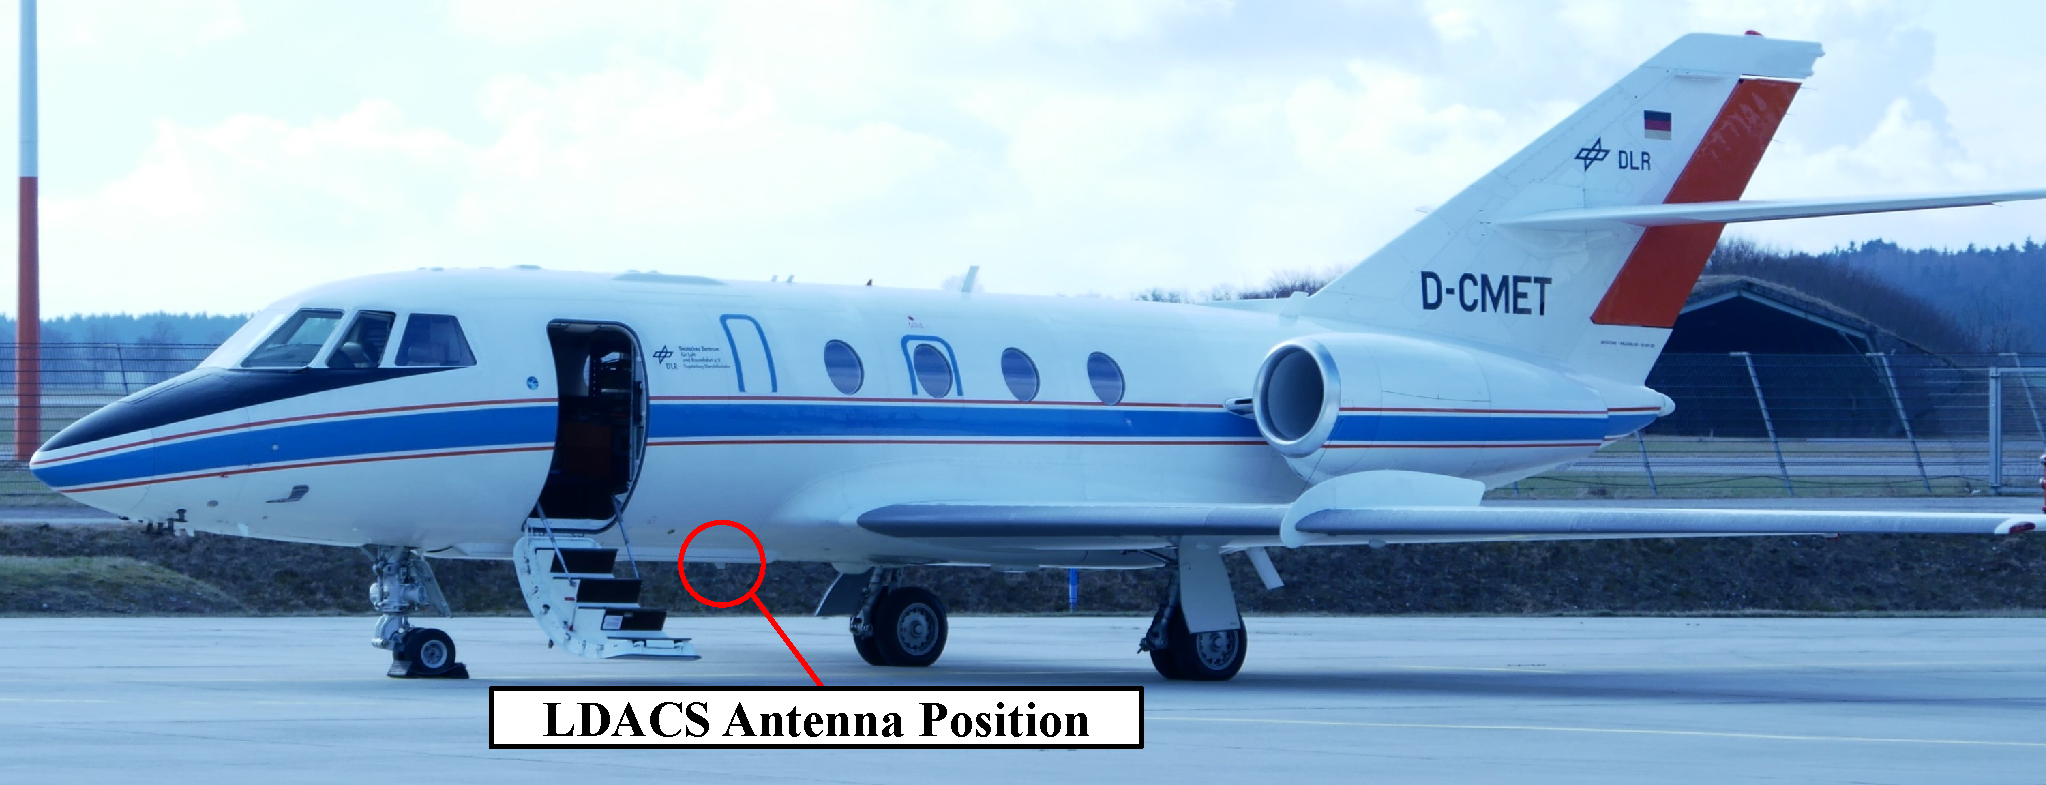
\includegraphics[width=0.99\linewidth]{img/Falcon-D20.pdf}
            \caption{Research aircraft used in the\\ experiments.}
            \label{fig:FalconD20E5}
    \end{subfigure}%
	\begin{subfigure}[b]{0.245\columnwidth}
        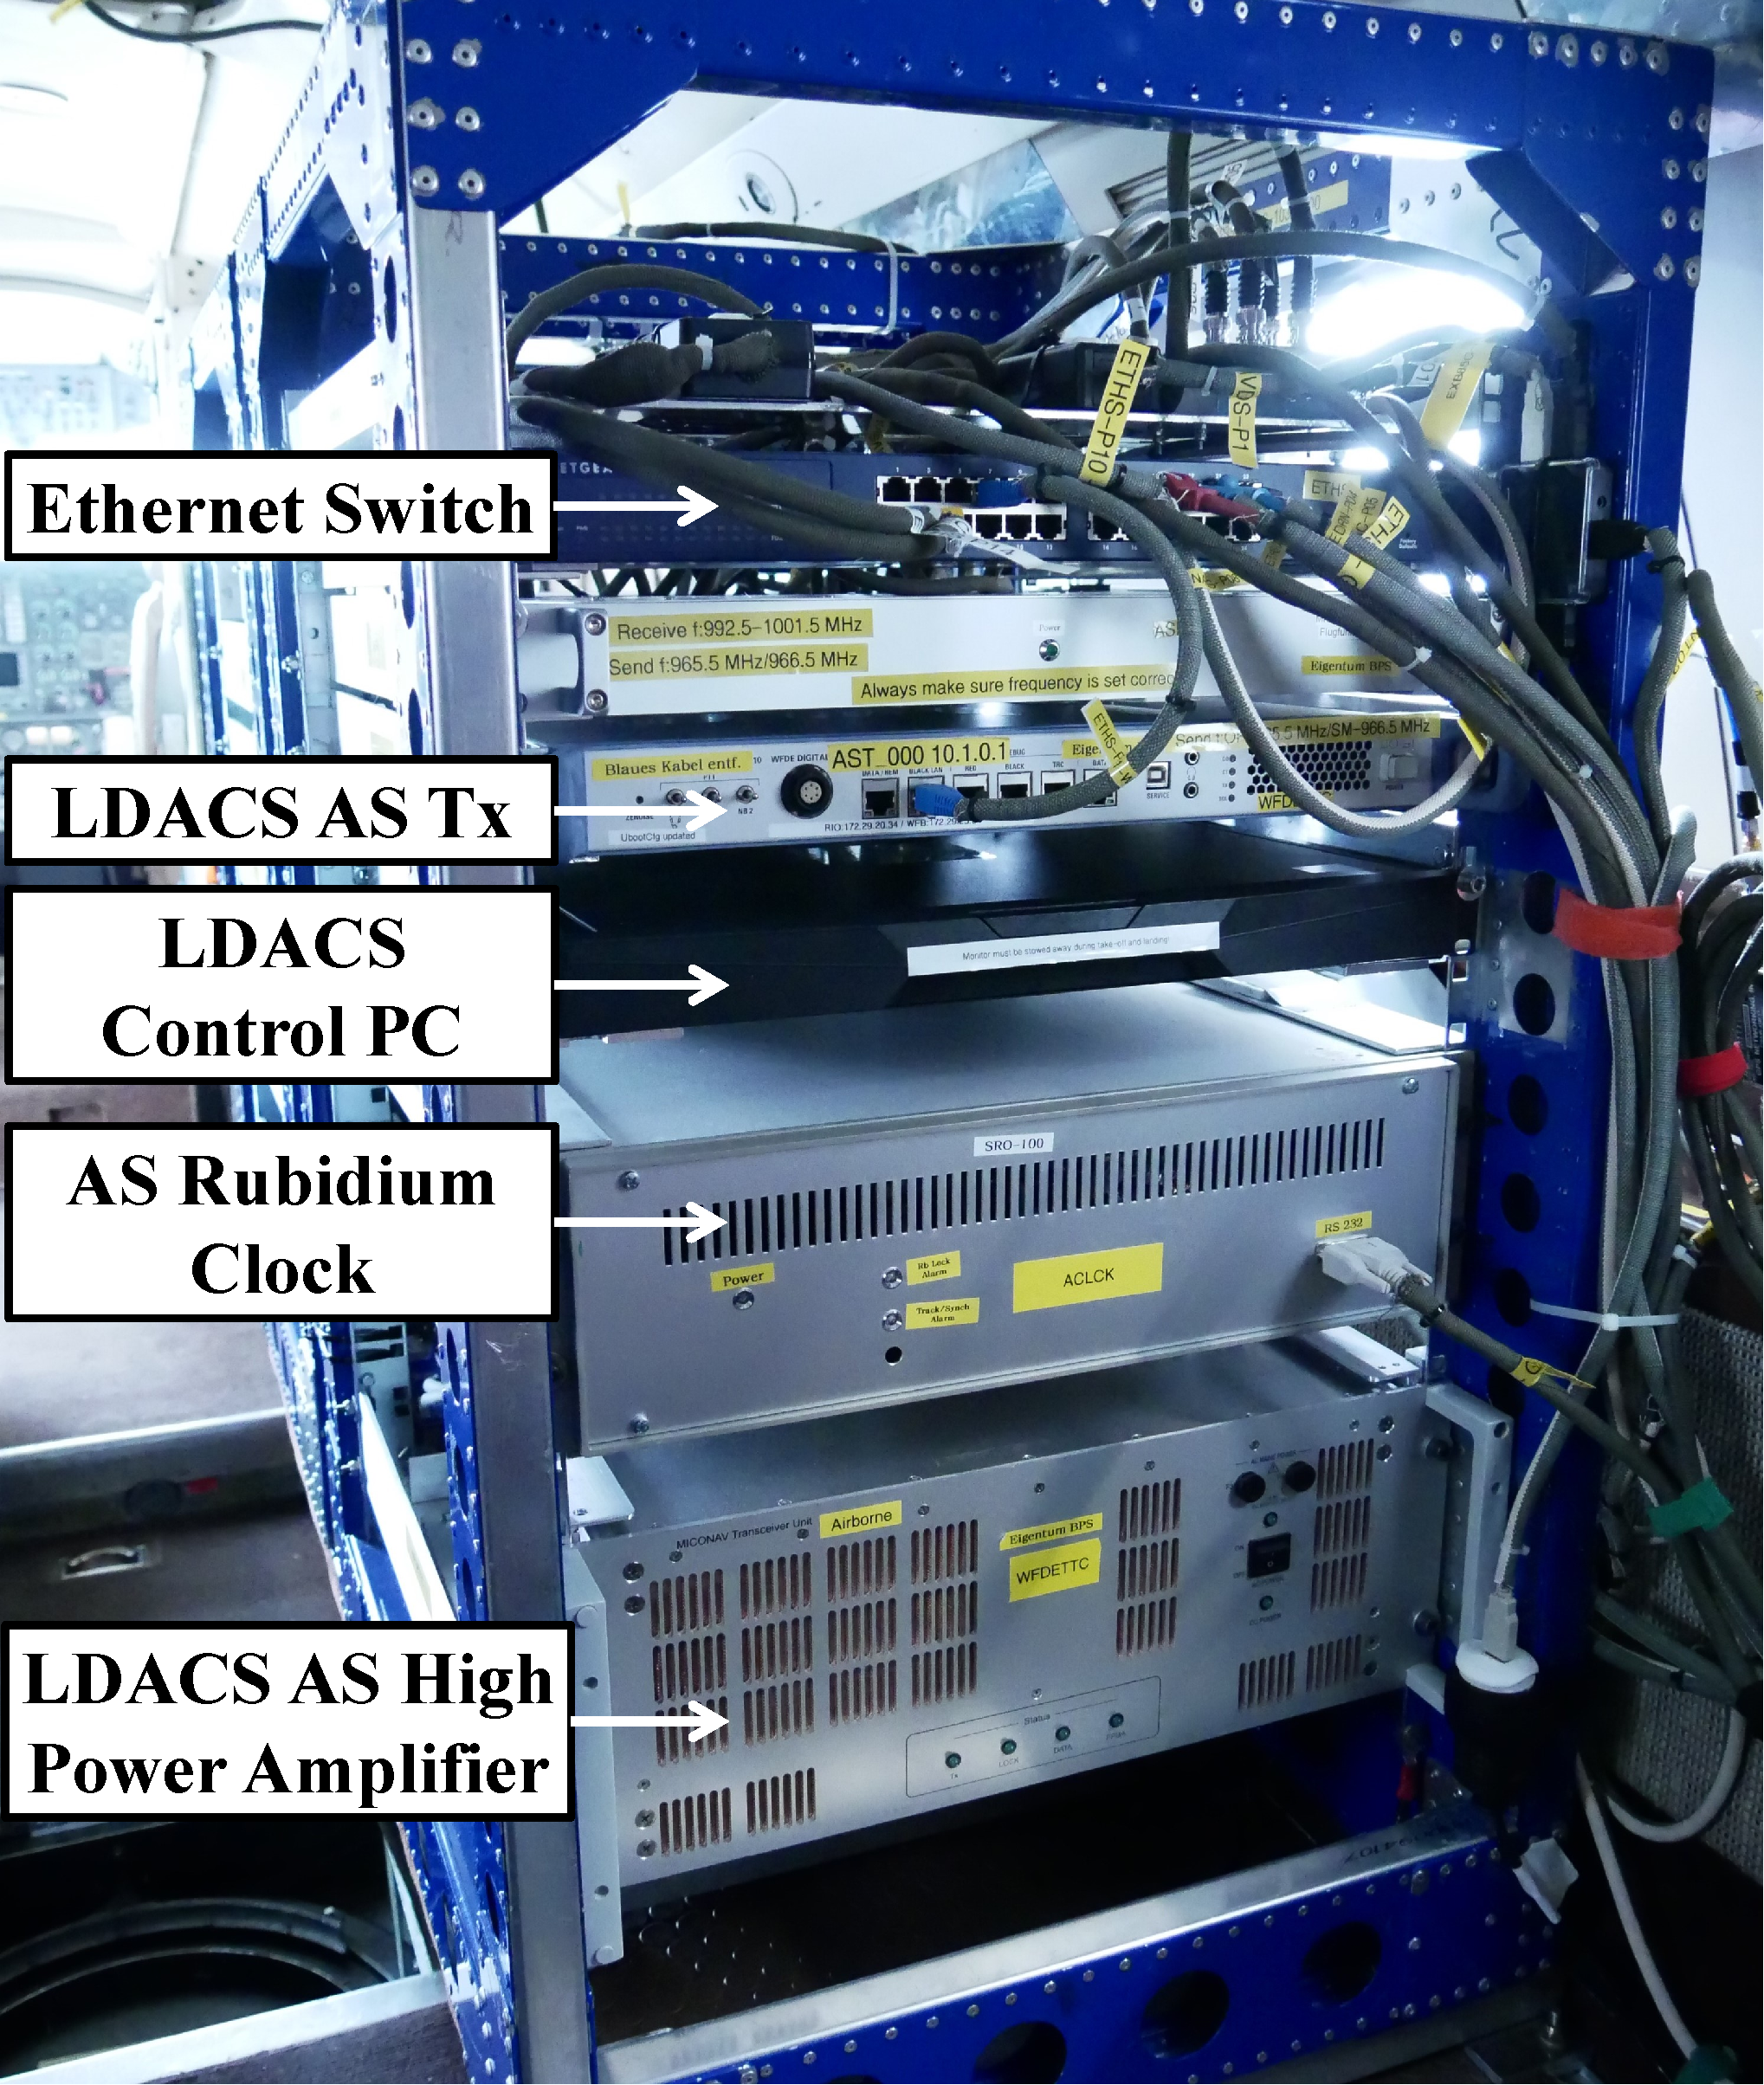
\includegraphics[width=0.99\linewidth]{img/AirborneStation.pdf}
        \caption{Airborne \\ equipment.}
        \label{fig:AirborneEquipment}
    \end{subfigure}
    \caption{LDACS experimental flight equipment.}
    \label{fig:flights}
\end{figure}

It supports \ac{ATS} and \ac{AOC} applications. It has been designed with future applications in mind, such as 4D trajectory management, and offers therefore at least 10 times more net capacity than the currently used terrestrial link i.e.\ the \ac{VDLm2} \cite{graeupl2019}. Instead of kilobits per second, LDACS offers up to 2 Mbps. By enabling not only communication but also navigation and surveillance through the use of the same radio signals, it is the world's first integrated \ac{CNS} system \cite{schnell2019}.

The LDACS network is comprised of several radio cells and is controlled by one \ac{GSC}. Each radio cell has a transmission site, called a \ac{GS} and can serve up to 512 \ac{AS}. This is illustrated in Figure \ref{fig:figure1}.

\begin{figure}
		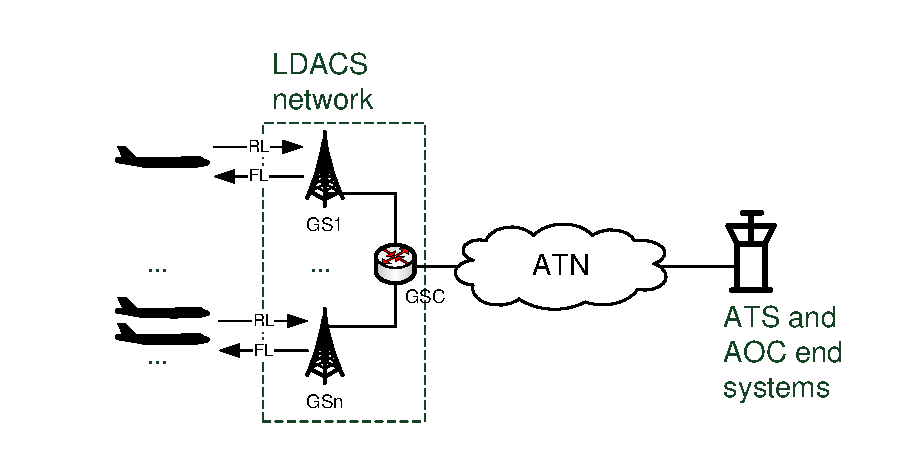
\includegraphics[width=\columnwidth]{img/figure_1.pdf}
		 \caption{LDACS network architecture: \ac{AS} connect to LDACS \ac{GS} controlled by a \ac{GSC}. The GSC connects the LDACS sub-network to the global \ac{ATN} to which the corresponding \ac{ATS} and \ac{AOC} end systems are attached.}
 	\label{fig:figure1}
\end{figure}

In \cite{maeurer20181} the initial LDACS's cybersecurity architecture was analyzed, leading to an updated cybersecurity architecture and integration of new algorithms as published in \cite{maeurer20182,  maeurer20191}. The approach was successfully evaluated in \cite{maeurer20192} and provides the baseline for this work.
